\section{Erfassung der Daten und Aufbereitung}
\label{sec:erfassung}
In diesem Abschnitt wird beleuchtet, wie die für die Verifikation der Hypothesen notwendigen Daten erfasst werden können.
Gegebenenfalls müssen die Daten für eine Analyse ebenfalls vorverarbeitet werden, um einen brauchbaren Datensatz zu erhalten.
Die Qualität der zugrunde liegenden Daten bestimmt die Aussagekraft, mit der die Hypothesen verifiziert oder verworfen werden können.

Für die Analyse eignen sich Open Source Projekte,
da diese sowohl den Quellcode als auch verschiedene Issue-Tracker,
in denen Sicherheitslücken gelistet sind,
öffentlich zugänglich machen.
In den Arbeiten von Chowdhury und Zulkernine wird \emph{Mozilla Firefox} als Gegenstand der Fallstudien verwendet~\cite{chowdhury_zulkernine_2010,chowdhury_zulkernine_2009}.
Die Festlegung auf ein einziges Projekt limitiert jedoch die Aussagekraft der Studie.
Daher haben Alves et al. mehrere Projekte für ihre Studie ausgewählt~\cite{alves_et_al}: 
Mozilla Projekte (Firefox, Thunderbird und andere),
den Linux Kernel,
den \emph{Xen} Hypervisor,
den Apache Webserver \texttt{httpd} und
die GNU Bibliothek \texttt{glibc}.

Informationen über Sicherheitslücken lassen sich über sog. \emph{Security Advisories} erhalten.
Diese listen entdeckte Bugs in der Software auf, die einen sicherheitsbezogenen Kontext haben.
Ein Eintrag in einer diesem Advisories enthält Informationen über die Sicherheitslücke, eine Bewertung der Schwere dieser Lücke und einen Link zu dem entsprechenden Bug-Tracker-Eintrag.
Abbildung \ref{fig:mfsa} zeigt einen Eintrag auf der \textit{Mozilla Foundation Security Advisories}\footnote{\url{https://www.mozilla.org/en-US/security/advisories/}} Webseite, die von verschiedenen Forschern verwendet wird~\cite{alves_et_al,chowdhury_zulkernine_2010}.
Für viele andere Projekte existieren ebenfalls Security Advisories.
\begin{figure}
	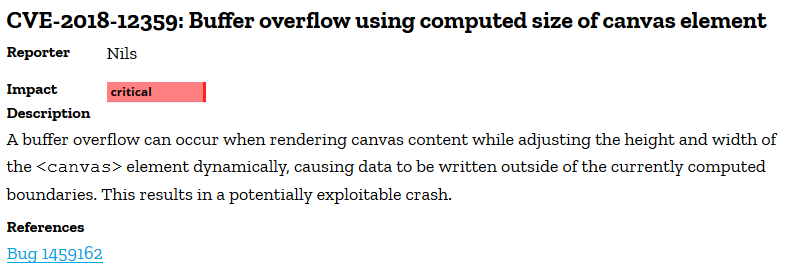
\includegraphics[width=\textwidth]{img/mfsa_example.png}
	\caption{Beispieleintrag auf der \textit{Mozilla Foundation Security Advisories} Webseite}
	\label{fig:mfsa}
\end{figure}

Für die statische Codeanalyse wird der Quellcode in zwei Versionen benötigt, nämlich vor und nach dem Beheben einer Sicherheitslücke.
Auf beiden Version wird die Codeanalyse ausgeführt, um die Metriken zu berechnen.
Durch die Unterschiede in den Metriken lässt sich ermitteln, was das Beheben einer Sicherheitslücke in den Metriken bewirkt.

Über die Security Advisories und den Bug Trackern lassen sich die Versionen bzw. Commits finden, in denen die Sicherheitslücken geschlossen wurden.
Dafür werden Parser-Programme verwendet, die die aufgelisteten Sicherheitslücken durchsuchen und die Referenzen auf die Versionen bzw. Commits der Behebungen ermitteln~\cite{alves_et_al,chowdhury_zulkernine_2009}.
Da die Einträge nicht immer konsistent gehalten werden, erschwert dies die Arbeit der Parser.
Alves et al. konnten daher nur 55 \% der Einträge in den untersuchten Projekten verarbeiten~\cite{alves_et_al}.
Das lässt viele Sicherheitslücken aus und mindert daher die Menge geeigneter Daten.

Ist die Version einer Software gefunden, in der eine Sicherheitslücke geschlossen wurde, kann die statische Codeanalyse durchgeführt werden.
Für einen Vergleich der Metriken muss eine andere Version ebenfalls analysiert werden, bestenfalls der Commit, der direkt vor dem Schließen der Lücke steht.
Alves et al. nehmen hierfür den Commit, der sich direkt davor in der Historie verwendet.
Es besteht allerdings die Möglichkeit, dass eine Lücke in mehreren Commits bearbeitet wird.
Der letzte Commit könnte beispielsweise nur "`Schönheitskorrekturen"' beinhalten, die keinerlei Auswirkungen auf die Metriken haben.
Ebenso ist es denkbar, dass der Hauptzweig kurz vor Schließung der Sicherheitslücke gemerged wurde.
Dann enthält dieser Commit potentiell sehr viele Änderungen, die nicht in Verbindung mit der Sicherheitslücke stehen.
Damit wären die Metriken sehr verschieden.
Chowdhury und Zulkernine verwenden für ihre Studie Release-Versionen von Mozilla Firefox.
Diese Herangehensweise ist kritisch zu betrachten, da damit die Ergebnisse der Codeanalyse verfälscht werden können.
Release-Versionen beinhalten in der Regel viele Änderungen, sodass die Metriken keinen Bezug zur Sicherheitslücke haben.

Die Erfassung der Metriken kann auf verschiedenen Ebenen erfolgen, beispielsweise auf Klassenebene oder Funktionsebene.
Eine einfache Art stellt die Dateiebene dar.
Sie ist universell für alle Arten von Software-Systemen.
Für andere Ebenen ist es notwendig, die Dateien zu parsen.
Unterschiedliche Sprachen bieten auch unterschiedliche Gruppierungsmechanismen an.
In C gibt es beispielsweise keine Klassen.
Deshalb wird in der Arbeit von Alves et al. bei den Projekten, die in C geschrieben wurden, \texttt{Structs} und \texttt{Unions} wie Klassen in C++ behandelt.

Bei Verwendung der Dateiebene für die Erfassung der Metriken muss bedacht werden, wie sich der Wert einer Datei aus den analysierten Elementen zusammensetzt.
Befinden sich in einer Datei beispielsweise zwei Klassen mit unterschiedlichen Metrik-Werten, müssen diese Werte zusammengefasst werden.
Eine Möglichkeit die Werte zusammenzufassen ist das arithmetische Mittel zu berechnen~\cite{chowdhury_zulkernine_2009}.
Alternativ dazu kann man auch das Maximum bilden.
Analoges gilt bei der Erfassung von Metriken auf Klassenebene unter Einbeziehung der jeweiligen Methoden der Klasse.

Die Wahl des Programms zur Berechnung der Metriken hängt von der Analyse ab, die anschließend mit den Metriken vorgenommen werden soll.
Nicht jedes Programm kann alle gewünschten Metriken berechnen und eigene Implementationen sind zeitaufwendig.
In den Studien von Alves et al. und Chowdhury und Zulkernine kam dafür das Tool \emph{Understand}\footnote{Understand Webseite: \url{https://scitools.com/features/}} zum Einsatz~\cite{alves_et_al,chowdhury_zulkernine_2009}.
Damit konnten alle benötigten Metriken für die Analyse erfasst werden, wenn auch einige wünschenswerte Metriken fehlten.
